\label{casestudy-def-chapter}
%\section{Security Definition of mCertiKOS}
%\label{casestudy-def}

We will now discuss how to apply the methodology of
Chapters~\ref{informal-chapter} and~\ref{methodology-chapter} to
formally guarantee end-to-end isolation between user 
processes running on top of the mCertiKOS kernel~\cite{certikos-popl}. 
During the proof effort, we had to make some changes to the operating
system to close potential security holes. We refer to our secure 
variant of the kernel as mCertiKOS-secure.

\section{mCertiKOS Overview}

The starting point for our proof effort was the basic version of
the mCertiKOS kernel, described in detail in Section~7 
of~\cite{certikos-popl}. We will give an overview of the kernel
here. It is composed of $32$ abstraction \emph{layers},
which incrementally build up the concepts of physical memory
management, virtual memory management, kernel-level processes,
and user-level processes. Each layer $L$ consists of the
following components:
\begin{itemize}
\item a type $\Sigma_L$ of program state, separated into 
machine registers, concrete memory, and abstract data of type $D_L$
\item a set of initial states $I_L$ and final states $F_L$
\item a set of primitives $P_L$ implemented by the layer
\item for each $f \in P_L$, a deterministic specification of type
$\Sigma_L \to \option{\Sigma_L}$
\item \textit{(if $L$ is not the bottom layer)} for each  
$f \in P_L$, an implementation written
in either LAsm$(L')$ or ClightX$(L')$ (defined below), where 
$L'$ is the layer below $L$
\item two special primitives called \ttt{load} and \ttt{store}
that model access to global memory; these primitives have no 
implementation as they are a direct model of how the x86 machine
translates virtual addresses using page tables
\end{itemize}

The top layer is called TSysCall, and the bottom is called
MBoot. MBoot describes execution over the model of the actual hardware;
the specifications of its primitives are taken as axioms. Implementations
of primitives in all layers are written in either a layer-parameterized
variant of x86 assembly or a layer-parameterized variant of C. 

The assembly language, called LAsm$(L)$, is an extension of 
CompCert's~\cite{compcert} model of x86 assembly that allows primitives
of layer $L$ to be called atomically. When an atomic primitive call
occurs, the semantics consults that primitive's specification
to take a step. Note that the \ttt{load} and \ttt{store} primitives are never
called explicitly (as they have no implementation), but instead
are used to specify the semantics of x86 instructions that read or
write memory (e.g., \ttt{movl \%eax, 0(\%ecx)}).

The C variant, called ClightX$(L)$, is an extension of
CompCert's Clight language~\cite{blazy-leroy-clight} (which is a 
slightly-simplified version of C). Like LAsm$(L)$, the semantics
is extended with the ability to call the primitives of $L$
atomically. ClightX$(L)$ programs can be compiled to LAsm$(L)$
in a verified-correct fashion using the CompCertX 
compiler~\cite{certikos-popl}, which is an extension of 
CompCert\ifextended~that supports per-function compilation\else\fi.

Each layer $L$ induces a machine $M_L$ of the kind described in
Section~\ref{methodology-machine}\ifextended. The state type and initial/final states
of $M_L$ come directly from $L$. The transition relation of
type $\pwrset{\Sigma_L \times \Sigma_L}$ is precisely the operational 
semantics of LAsm$(L)$. The machine's observation function will be 
discussed later, as it is an extension that we implemented over
the existing mCertiKOS specifically for the security proof.
\else, with transition relation defined
by the operational semantics of LAsm$(L)$.
\fi

\begin{comment}
\paragraph{Load/Store Primitives}
Before continuing, there is one somewhat technical detail 
regarding the LAsm$(L)$ semantics that requires explanation. 
While most layer primitives are called in LAsm$(L)$ using 
the \ttt{call} syntax, the special \ttt{load} and \ttt{store}
primitives work differently. Whenever an
assembly command dereferences an address, the LAsm$(L)$
semantics consults the load/store primitives to decide 
how the dereference is actually resolved. 
As an example, consider the following snippet
of assembly code, taken from the implementation of the
page fault handler TSysCall primitive:
{\small
\begin{alltt}
   call trap_get
   movl \%eax, 0(\%esp)   
   call ptfault_resv
\end{alltt}
}
\noindent
The layer below TSysCall is called TDispatch, and thus this
code is written in the language LAsm(TDispatch).
The first and third lines call primitives of TDispatch
atomically. The second line ostensibly writes the value 
of EAX into the memory location pointed to by ESP. The 
actual semantics of this line, however, will call
TDispatch's \ttt{store} primitive with the value of EAX and the
address in ESP as parameters. This primitive will
translate the destination address from virtual to physical
by walking through the page tables of the currently-executing
process.
\end{comment}

\begin{figure}
\centering{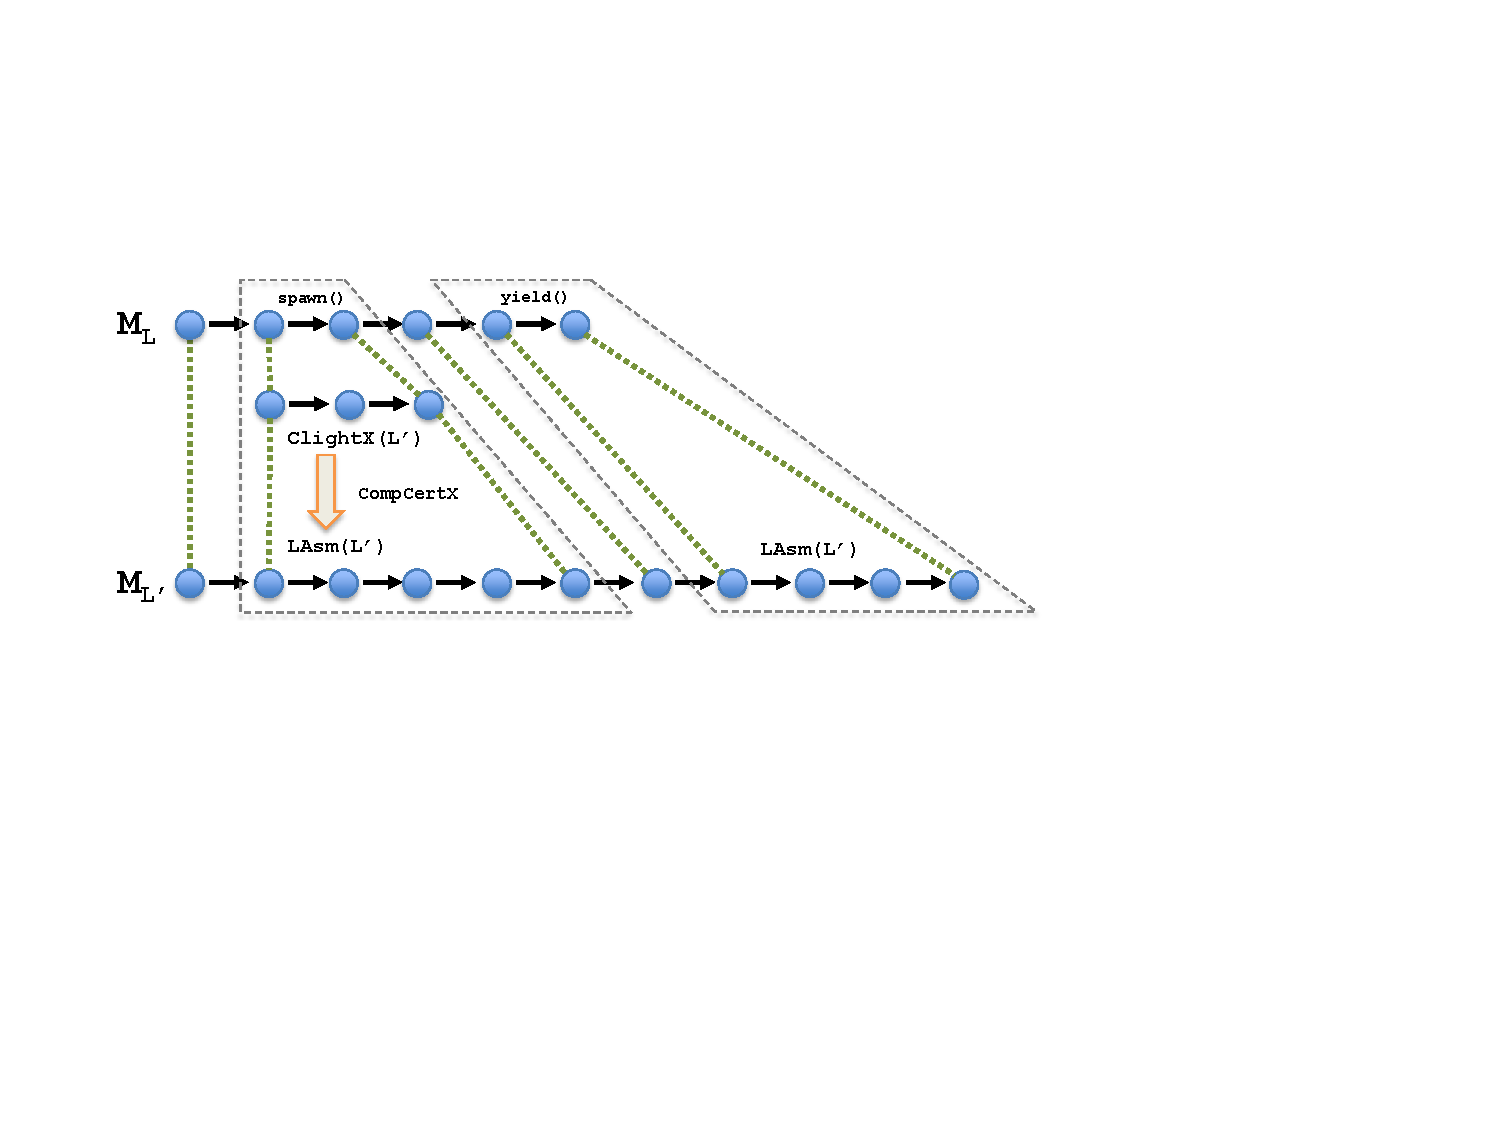
\includegraphics[scale=0.53]{pldi/figure/layer-sim.pdf}}
\caption{\small{Simulation between adjacent layers.
Layer $L$ contains primitives \ttt{spawn} and \ttt{yield},
with the former implemented in ClightX$(L')$ and the latter
implemented in LAsm$(L')$.}}
%\vspace*{-2ex}
\label{layer-sim}
\end{figure}

\paragraph{Layer Simulation}
Figure~\ref{layer-sim} illustrates how machines induced by two 
consecutive layers are connected via simulation. Each step 
of machine $M_L$ is either a standard assembly command
or an atomic primitive call. Steps of the former category are
simulated in $M_{L'}$ by exactly the same assembly command.
Steps of the latter are simulated using the primitive's 
implementation, supplied by layer $L$. If the primitive is
implemented directly in LAsm$(L')$ (e.g., \ttt{yield} in Figure~\ref{layer-sim}), 
then the simulation directly 
uses the small-step semantics of this implementation. If the primitive is
implemented in ClightX$(L')$ (e.g., \ttt{spawn} in Figure~\ref{layer-sim}), 
then CompCertX's compilation is inserted into the simulation. CompCertX is
verified to provide a simulation from the ClightX$(L')$
execution to the corresponding LAsm$(L')$ execution, so 
this is chained appropriately to get an end-to-end
simulation from the $M_L$ execution to the $M_{L'}$
execution.

As a general convention, the simulation relation between 
consecutive machines only represents an abstraction of
some concrete memory into abstract data. In other words,
some portion of concrete memory in the lower-level machine is related
to some newly-introduced portion of abstract data in the higher-level 
machine. In this way, as we move up the layers, concrete memory gets
incrementally abstracted away in a monotonic fashion.
Once we reach the top layer, TSysCall, 
concrete memory has been fully abstracted away from user-mode
semantics; hence user processes have no mechanism for interacting
with the concrete memory directly. In fact, by convention, 
mCertiKOS actually requires that primitive specifications
at \emph{all} layers do not interact with concrete memory.
If a primitive needs to access some portion of concrete memory,
then a layer must first be introduced to abstract that memory.

Once every pair of consecutive machines is connected with a
simulation, they are combined transitively to 
obtain a simulation from TSysCall to MBoot. Since the TSysCall layer
provides mCertiKOS's system calls as primitives, user process
execution is specified at the TSysCall level.
To get a better sense of user process execution, we will now 
describe the abstract data and primitives of the TSysCall layer 
in mCertiKOS-secure.

\begin{comment}
\begin{figure}
\centering{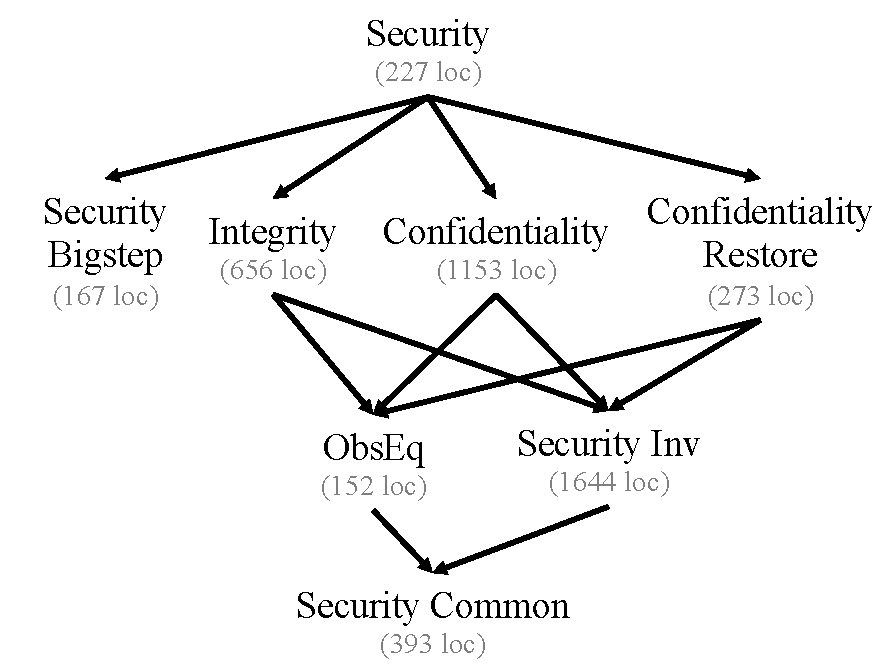
\includegraphics[scale=0.5,origin=c]{figure/code_structure.pdf}}
\caption{\small{Dependencies and line counts of security-related proofs. Note 
that most of the new invariants in SecurityInv were needed for
confidentiality, so the relative effort required for proving
confidentiality is larger than it appears from the line counts.}}
\label{files}
\end{figure}

The entire Coq code base of mCertiKOS-secure can be found in the
supplementary material~\cite{costanzo-popl16-tr}. The security proof
can be found within the \ttt{security} directory. Figure~\ref{files}
names all of the relevant Coq files in the \ttt{security} directory,
and shows their dependency relations and line counts ignoring blank
lines. This figure can be used to maintain a high-level understanding
of the proof structure as we delve into the proof details throughout
this section and the next.
\end{comment}

\paragraph{TSysCall State}
The TSysCall abstract data is a Coq record consisting of $32$
separate fields. We list here those fields that will be
relevant to our discussion later. In the following, whenever a field 
name has a subscript of $i$, the field is a finite map from 
process ID to some data type. Each user process running over the
kernel has a unique, integer-valued process ID, and IDs are never
reused. From a security standpoint, one should think of each process
ID value as a unique principal or security domain.

\begin{itemize}
\item $\ttt{out}_i$~--- The output buffer for process $i$\ifextended,
represented as a list of $32$-bit integers\else\fi.
Note that output buffers
exist in all layers' abstract data, including MBoot. They are
never actually implemented in memory; instead, they are assumed to be
a representation of some external method of output (e.g., a monitor
or a network channel), and are used to define the observable
events of user-process execution.
\ifextended
\item $\ttt{ikern}$~--- A global boolean flag stating whether
the machine is currently in kernel mode or user mode.
\else\fi
\item $\ttt{HP}$~--- A global, flat view of the user-space
memory heap\ifextended~(physical addresses between $2^{30}$ and 
$3 \times 2^{30}$)\else\fi.
A \emph{page} is defined as the $4096$-byte sequence starting 
from a physical address that is divisible by $4096$.
\item $\ttt{AT}$~--- A global allocation table, represented as
a bitmap indicating which pages in the global heap have been 
allocated. Element $n$ corresponds to 
\ifextended
the $4096$-byte page starting from physical address $4096n$.
\else page $n$. 
\fi
\item $\ttt{pgmap}_i$~--- A representation of the two-level page 
map for process $i$. The page map tells the x86 machine how
to translate virtual addresses between $0$ and $2^{32} - 1$ into 
physical addresses.
\item $\ttt{container}_i$~--- Metadata for process $i$
regarding spawned status, children,
parents, and resource quota. A container is itself a 
Coq record containing the following fields:
\begin{itemize}
\item $\ttt{used}$~--- A boolean indicating whether process $i$ has
been spawned.
\item $\ttt{parent}$~--- The ID of the parent of process 
$i$\ifextended~(or $0$ for root process $0$)\else\fi.
\item $\ttt{nchildren}$~--- The number of children of process $i$.
\item $\ttt{quota}$~--- The maximum number of pages that process
$i$ is allowed to allocate.
\item $\ttt{usage}$~--- The current number of pages that process
$i$ has allocated.
\end{itemize}
%There are a number of invariants maintained that guarantee the
%container structure forms a valid tree. Furthermore, a process's
%quota is always at least as large as the sum of its childrens'
%quotas, meaning that the root (process $0$) quota provides an
%upper bound for the whole system.
\item $\ttt{ctxt}_i$~--- The saved register context of 
process $i$, containing the register values that will need to 
be restored the next time process $i$ is scheduled.
\item $\ttt{cid}$~--- The currently-running process ID.
\ifextended
\item $\ttt{rdyQ}$~--- An ordered list of process IDs that are
ready to be scheduled (head of the list is the next to be scheduled).
\else\fi
\end{itemize}

\noindent
Note that process containers, which track parent/child relationships
and dynamic resource usage, did not exist in the initial version of 
mCertiKOS taken from~\cite{certikos-popl}. Prior to conducting
our security proof, we realized that a lack of dynamic resource
tracking would be extremely problematic for security, since a
user process could easily affect others via a denial-of-service
attack that repeatedly allocates pages until all of physical memory
is exhausted. Therefore, inspired by the concept of containers
in the HiStar security-aware operating system~\cite{histar}, we
chose to implement a similar notion of container objects in 
mCertiKOS to preemptively deal with this security issue. Containers
not only enforce a quota on the number of memory pages each process 
is allowed to dynamically allocate, but they also allow processes to
distribute some of their memory quota to children. In 
Chapter~\ref{casestudy-proof-chapter}, we will illustrate  
how containers and memory quotas are crucial to our security proof.

\paragraph{TSysCall Primitives}
There are $9$ primitives in the TSysCall layer of mCertiKOS-secure, including the
load/store primitives. The primitive specifications operate over
both the TSysCall abstract data and the machine registers.
Note that they do not interact with concrete memory since all 
relevant portions of memory have already been abstracted
into the TSysCall abstract data.

\begin{itemize}
\item \emph{Initialization}~--- \ttt{proc\_init} sets up the various kernel 
objects to get everything into a working state. We never attempt to 
reason about anything
that happens prior to initialization; it is assumed that the bootloader
will always call \ttt{proc\_init}.
\item \emph{Load/Store}~--- Since paging is enabled in all user-mode 
TSysCall states, the \ttt{load} and \ttt{store} primitives walk the 
two-level page table of the currently-running process to
translate a virtual address into physical. If no physical address is
found due to no page being mapped, then the faulting virtual address is
written into the CR2 control register, the current register context
is saved, and the instruction pointer register is updated to point to 
the entry of the page fault handler primitive.
\item \emph{Page Fault}~--- \ttt{pgf\_handler} is called immediately after one 
of the load/store primitives fails to resolve a virtual address. It reads
the faulting virtual address from the CR2 register, allocates one or two 
new pages as appropriate, increases the current process's page usage
(see the \ttt{container} description above),
and plugs the page(s) into the page table.
It then restores the register context that was saved when the 
load/store primitive faulted. If the current process does not
have enough available quota to allocate the required pages, then
the instruction pointer register is updated to point to the entry
of the yield primitive (see below). \cut{This means that the process will
end up page faulting and yielding infinitely.}
\item \emph{Get Quota}~--- \ttt{get\_quota} returns the amount of remaining 
quota for the currently-executing process. This is useful to provide
as a system call since it allows processes to divide their
quota among children in any way they wish.
\item \emph{Spawn Process}~--- \ttt{proc\_create} attempts to spawn a new 
child process. It takes a quota as a parameter, specifying the maximum number 
of pages the child process will be allowed to allocate. This quota allowance 
is taken from the current process's available quota.
\item \emph{Yield}~--- \ttt{sys\_yield} performs the first step for 
yielding\cut{ to the next process in the ready queue}. 
It enters kernel mode, disables paging, saves the current registers, and changes
the currently-running process ID to the head of the ready queue (updating
the ready queue accordingly). It then 
context switches by restoring the newly-running process's registers. The 
newly-restored instruction pointer register is guaranteed (proved as an invariant) to 
point to the function entry of the \ttt{start\_user} primitive.
\item \emph{Start User}~--- \ttt{start\_user} performs the simple second step
of yielding. It enables paging for the currently-running process and exits
kernel mode. The entire functionality of yielding must be split into
two primitives (\ttt{sys\_yield} and \ttt{start\_user}) because
context switching requires writing to the instruction pointer register,
and therefore only makes sense when it is the final operation performed by
a primitive. 
Hence yielding is split into one primitive that ends with a 
context switch, and a second primitive that returns to user mode.
\item \emph{Output}~--- \ttt{print} appends its integer parameter to the
output buffer of the currently-running process.
\end{itemize}

\section{Security Overview}
\label{ssec:security-overview}

\cut{We have now provided enough background on mCertiKOS to begin discussing
the security verification.}
We consider each process ID to be a
distinct principal\cut{ or security domain}. 
The security property that we aim to prove is exactly the high-level
security defined in Section~\ref{methodology-security} 
(Definition~\ref{high-level-security}), applied over the TSysCall machine 
using a carefully-constructed observation function that we define below. 
Theorem~\ref{end-to-end} then guarantees security of 
the corresponding whole-execution behaviors over the MBoot machine 
(which represents our lowest-level model of the assembly machine).

\paragraph{High-Level Semantics}
\ifextended
As explained in Chapters~\ref{informal-chapter} and~\ref{methodology-chapter},
high-level
\else
High-level \fi 
security is proved by showing that every step of
execution preserves an indistinguishability relation saying 
that the observable portions of two states are equal. In
the mCertiKOS context, however, this property will not actually
hold over the TSysCall machine, because it models the
execution of \emph{all} user processes, not just the observer's process.

To see this, consider any process ID $p$, which we
call the observer process. For any TSysCall state $\sigma$, we say
that $\sigma$ is ``active'' if \ttt{cid}$(\sigma) = p$, and
``inactive'' otherwise. Now consider whether the values in machine
registers should be observable to $p$. Clearly, if $p$ is executing,
then it can read and write registers however it wishes, so the
registers must be considered observable.  On the other hand, if some
other process $p'$ is executing, then the registers must be
unobservable to $p$ if we hope to prove that $p$ and $p'$ are
isolated. We conclude that registers should be observable to $p$ only
in active states.

What happens, then, if we attempt to prove that 
indistinguishability is preserved when starting from
inactive indistinguishable states? Since the states 
are inactive, the registers are unobservable, and so
the instruction pointer register in particular may have
a completely different value in the two states. This means
that the indistinguishable states may execute different
instructions. If, for example, one state executes the yield primitive
while the other does not, we may end up in a situation
where one resulting state is active but the other is not;
clearly, such states cannot be indistinguishable 
since the registers are observable in one state but not
in the other. Thus indistinguishability will not
be preserved in this example.

The fundamental issue here is that, in order to prove
that $p$ cannot be influenced by $p'$, we must show
that $p$ has no knowledge that $p'$ is even executing
over the kernel. We accomplish this by defining a
higher-level machine above the TSysCall machine, where every state 
is active, meaning the semantics itself hides the executions
of all processes except for the observer. We call this the TSysCall-local 
machine~--- it is parameterized by principal $p$, and it 
represents $p$'s local view of the TSysCall machine.

\begin{figure}
\centering{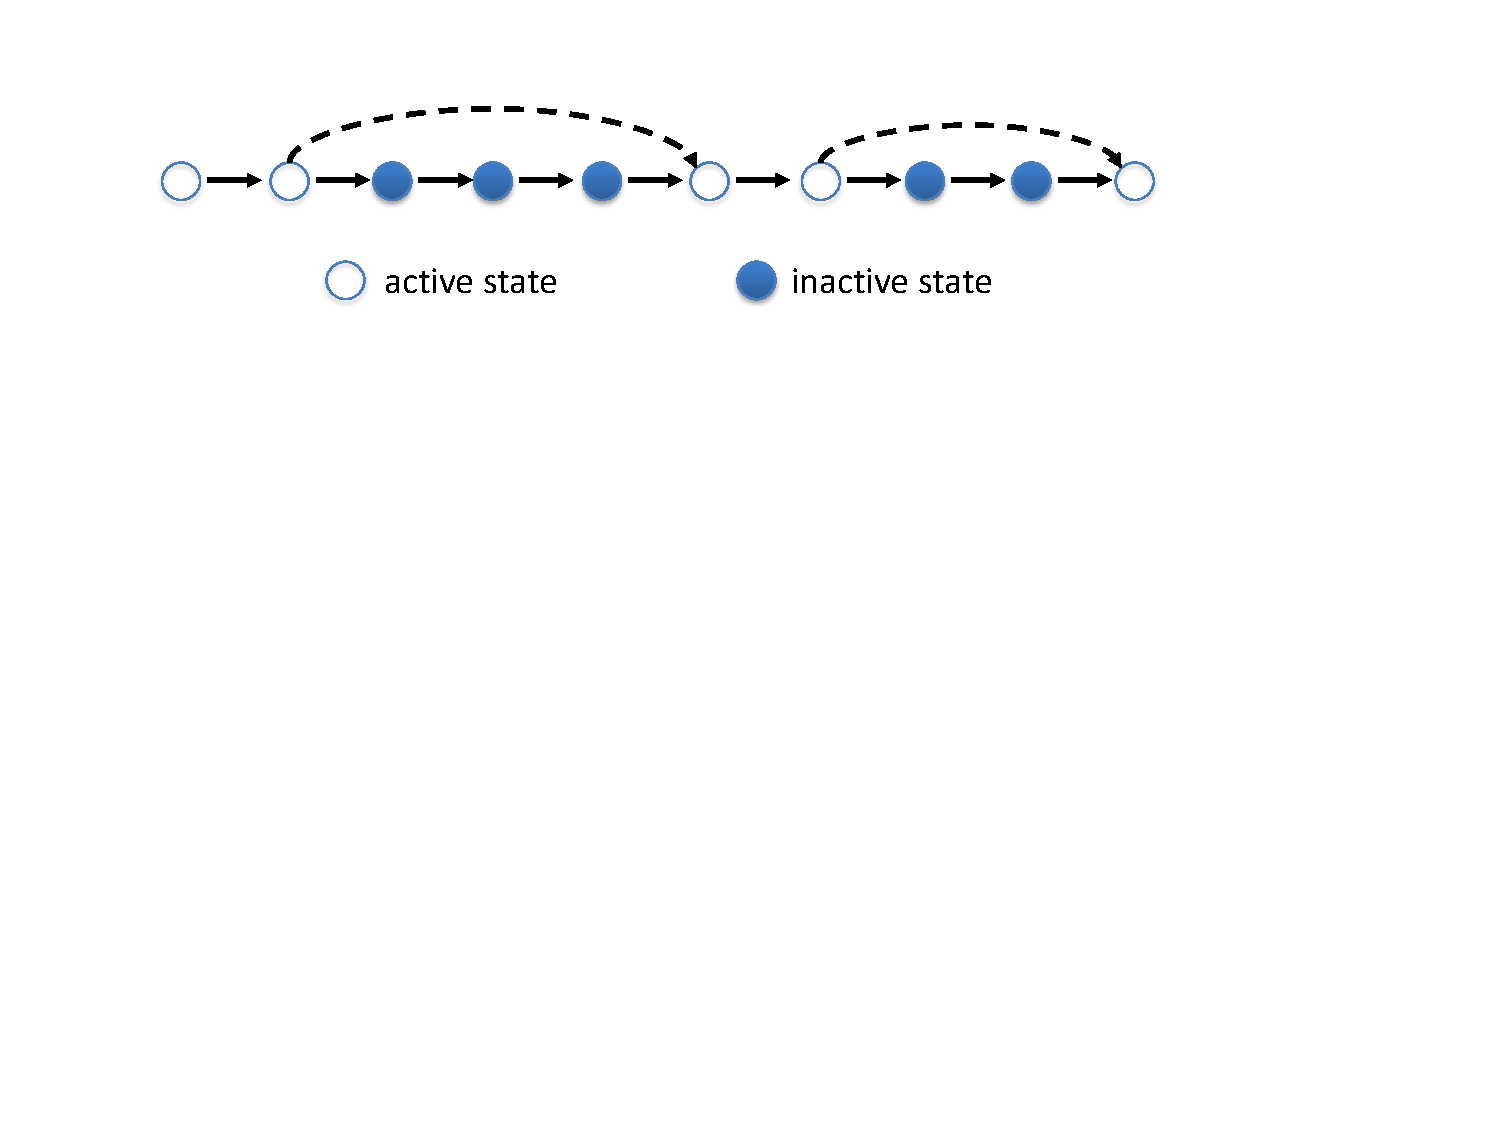
\includegraphics[scale=0.47]{pldi/figure/bigstep.pdf}}
\caption{\small{The TSysCall-local semantics, defined
by taking big steps over the inactive parts of the TSysCall 
semantics.}}
%\vspace*{-2ex}
\label{bigstep}
\end{figure}

Figure~\ref{bigstep} shows how
the semantics of
TSysCall-local is defined. The solid arrows are transitions of
the TSysCall machine, white circles are active TSysCall states, 
and shaded circles are inactive states. The TSysCall-local 
semantics is then obtained by 
combining all of the solid arrows connecting active states
with all of the dotted arrows. Note that in the TSysCall
layer, the yield primitive is the \emph{only} way that
a state can change from active to inactive, or vice-versa.
Thus one can think of the TSysCall-local machine as a
version of the TSysCall machine where the yield semantics
takes a big step over other processes' executions, immediately 
returning to the observer process that invoked the yield.

\ifextended
Given all of this discussion, our
\else Our \fi high-level security
property is proved over the TSys\-Call-local machine, for
\emph{any} choice of observer principal $p$. 
We prove simulation from TSysCall-local to 
TSysCall, so this strategy fits cleanly into our
security verification methodology.

\paragraph{Observation Function}

We now define the high-level observation function used
in our verification\cut{, which maps each principal and state
to an observation}. 
For a given process ID $p$, the state observation
of $\sigma$ is defined as follows:
\begin{itemize} \itemsep 0pt
\item \emph{Registers}~--- All registers are observable
if $\sigma$ is active. \cut{No registers are observable if 
$\sigma$ is inactive.}
\item \emph{Output}~--- The output buffer of $p$ is
observable.
\item \emph{Virtual Address Space}~--- We can dereference 
any virtual address by walking through $p$'s page tables.
This will result in a value if the address is actually
mapped, or no value otherwise. This function from virtual
addresses to option values is observable. Importantly,
the physical address at which a value resides is never
observable.
\item \emph{Spawned}~--- The spawned status of $p$ is observable.
\item \emph{Quota}~--- The remaining quota\cut{ (max quota minus usage)} 
of $p$ is observable.
\item \emph{Children}~--- The number of children
of $p$ is observable.
\item \emph{Active}~--- It is observable whether 
\ttt{cid}$(\sigma)$ is equal to $p$.
\item \emph{Reg Ctxt}~--- The saved register
context of $p$ is observable.
%\item \emph{Page Fault Info}~--- The CR2 register, which
%stores the offending virtual address after a page fault
%occurs, is observable whenever $p$ is active. We will 
%describe this point in some more detail later.
\end{itemize}

%%%%%%%%%%%%%%%%%%%%%%%%%%%%%%%%%%%%%%%%%%%%%%%%%%%%%%%%%%%%%%%%
\begin{figure}[t]
\begin{center}
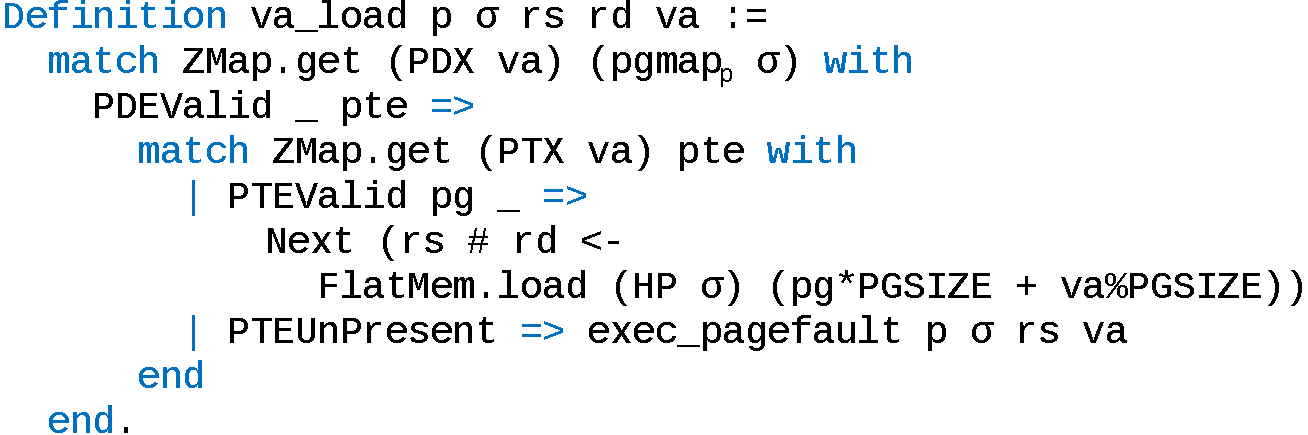
\includegraphics[scale=0.55]{pldi/figure/vaload}
\caption{\small Pseudocode of the \ttt{load} primitive
specification.}
\label{fig:va-load}
%\vspace*{-20pt}
\end{center}
\end{figure}
%%%%%%%%%%%%%%%%%%%%%%%%%%%%%%%%%%%%%%%%%%%%%%%%%%%%%%%%%%%%%%%%

The virtual address space component of the observation 
function is particularly interesting, as it showcases the
strength and generality of our methodology. Figure~\ref{fig:va-load}
shows pseudocode of the Coq specification used at the TSysCall 
level for loading data from the global heap (the \ttt{load}
primitive). The two \ttt{match} clauses walk the two levels
of page tables (\ttt{pgmap}) to convert a virtual address \ttt{va} 
into a physical page number \ttt{pg} and an offset
(assuming a page fault does not occur). The resulting
physical address, which we will refer to as \ttt{pa} in the
following, is computed as $\ttt{pg}*\ttt{PGSIZE} + \ttt{va}\%\ttt{PGSIZE}$.
Then \ttt{FlatMem.load} is called to obtain the value at location 
\ttt{pa} in the global heap \ttt{HP}. At first glance, it is
not at all obvious how one might prove the security of this 
specification. In particular, the value of \ttt{pa} causes
trouble: if the observer learns the physical address where his
data is located, he could potentially learn some information
about how other processes are allocating pages (e.g.,
the bigger the physical address, the more memory other processes
have been using). In traditional label-based reasoning, \ttt{pa}
would have a \hi{} security label, while the final data returned 
by the \ttt{FlatMem.load} lookup would have a \lo{} label. In other
words, \ttt{FlatMem.load} performs a \emph{declassification} here;
yet this declassification does not actually result in an information
leak. How can one prove that the declassification is acceptable?

Our verification methodology answers this question with ease. We
simply define our observation function as described above, so that
the physical address obtained during virtual address loading is 
unobservable. Only the following function is observed:
\[\observe{p}{\sigma} \quad \isdef \quad \ttt{fun} \ttt{ va} \Rightarrow
\ttt{va\_load}~p~\sigma~\ttt{va}\]
If we define the observation function in this way, and prove the 
high-level noninterference property (Definition~\ref{high-level-security})
with respect to this observation function, then we successfully 
guarantee that end-to-end behavior of \ttt{va\_load} really is 
independent from the specific value of \ttt{pa}. Hence our methodology
cleanly and implicitly shows that the declassification performed 
by \ttt{va\_load} is secure. Furthermore, this example demonstrates
the power of allowing the observation function to express more than
just a portion of program state. We define the observation to be
a subtle transformation involving both the
\ttt{pgmap} and \ttt{HP} portions of state.

\begin{comment}
\subsection{End-to-End Security}

We propagate the high-level security proof down to the 
MBoot layer by applying the end-to-end security theorem
of Section~\ref{methodology}. This requires proving that
the MBoot machine is both behavioral and deterministic. 
The proof of determinism is straightforward; it should not
be surprising that MBoot execution is deterministic since
the layer describes a direct model of hardware.

For behaviorality, we define the observation function of the MBoot
machine to be the output buffer (more precisely, for a given
principal $l$, the observation is $l$'s output buffer).
We then define a partial order over output buffers using a
standard list-prefix ordering~--- buffer $b$ precedes buffer
$b'$ iff $b$ is a prefix of $b'$. Behaviorality of MBoot is 
easy to prove with respect to this ordering, since the only 
way to modify the output buffer is to call the \ttt{print} 
primitive, which appends to the end of the buffer.

Note that, as described in Sections~\ref{informal} 
and~\ref{methodology}, we are also required to prove that
the simulation relation between TSysCall and MBoot is
compatible with the observation functions of the two layers,
in such a way that indistinguishability is preserved. We
prove this fact by first establishing that the output buffer
never changes across simulation of all layers: for every
pair of consecutive layers $L$ and $L'$ simulated with relation
$R$, we prove that the output buffers of any two states related
by $R$ are equal. Indistinguishability preservation is easy to
prove once we have established this fact. Recall the property
definition from Section~\ref{methodology}:
\begin{align*}
& \forall \sigma_1, \sigma_2 \in \Sigma_M, \,\, s_1, s_2 \in \Sigma_m \such \\
& \qquad \observem{M}{l}{\sigma_1} = \observem{M}{l}{\sigma_2} 
\land R(\sigma_1,s_1) \land R(\sigma_2,s_2) \\
& \qquad \Longrightarrow \observem{m}{l}{s_1} = \observem{m}{l}{s_2}
\end{align*}
Consider when $M$ is the TSysCall machine and $m$ is the MBoot machine.
Since we know that the simulation relation never changes the output
buffer, and the MBoot observation function is the output buffer, this
property reduces to showing that, for a given principal $l$, any two 
TSysCall states that are indistinguishable to $l$ have identical output 
buffers for $l$. This fact is obviously true since the TSysCall observation
function includes $l$'s output buffer as an observable component.
\else\fi
\end{comment}



